\section{Lead --- Wannier-interpolated Fermi surface}
\label{sec2:lead}
\begin{itemize}
\item Outline: {\it Obtain \MLWFs{} for the four lowest states in lead. Use Wannier interpolation to plot the
Fermi surface.}
\end{itemize}

\begin{figure}[h!]
\centering
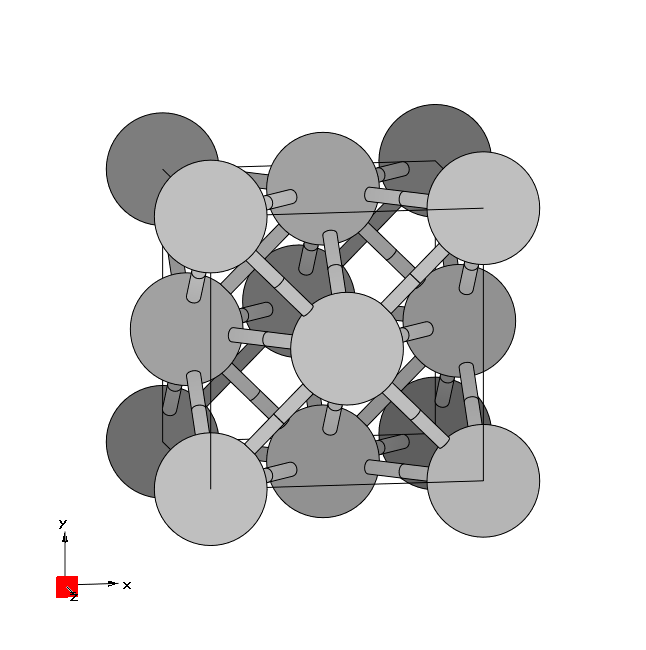
\includegraphics[width=0.25\columnwidth,trim={45pt 45pt 55pt 55pt},clip]{figure/example02/lead.png}
\caption{Unit cell of lead crystal plotted with the \xcrysden{} program.}
\label{fig2.0}
\end{figure}

\begin{enumerate}
\item {\it Inspect the output file {\tt lead.wout}.}

A summary of the wannierisation is given in tab.\ref{tab2.1}. At the end of the {\tt .wout} file you should find the info on the final state of the minimization as
\begin{tcolorbox}[sharp corners,boxrule=0.5pt]
{\small
\begin{verbatim}
 Final State
  WF centre and spread    1  (  0.397070,  0.397070,  0.397070 )     1.93781315
  WF centre and spread    2  (  0.397070, -0.397070, -0.397070 )     1.93781315
  WF centre and spread    3  ( -0.397070,  0.397070, -0.397070 )     1.93781315
  WF centre and spread    4  ( -0.397070, -0.397070,  0.397070 )     1.93781315
  Sum of centres and spreads (  0.000000, -0.000000, -0.000000 )     7.75125261

         Spreads (Ang^2)       Omega I      =     6.039099038
        ================       Omega D      =     0.007065754
                               Omega OD     =     1.705087819
    Final Spread (Ang^2)       Omega Total  =     7.751252611
 ------------------------------------------------------------------------------
\end{verbatim}
}
\end{tcolorbox}


\begin{table}[h!]
\centering
\caption{Converged values of the components of spread functional and their sum, given in \angsqd{}.}
\begin{tabular}{@{} lllll @{}}\toprule[1.5pt]
MP mesh & $\Omega$ & $\Omega\tinysub{I}$ & $\Omega\tinysub{OD}$ & $\Omega\tinysub{D}$ \\\midrule
$4\times4\times4$ & 7.751 &6.039 & 0.007 & 1.705 \\\bottomrule[1pt]
\end{tabular}\label{tab2.1}
\end{table}

\item {\it Use Wannier interpolation to generate the Fermi surface of lead.}

As can be seen from the bandstructure plot in the \Wannier{} tutorial, that we report here, \cf{} \Fig{fig2.1}, the four lower valence bands are separated in energy from the higher conduction states (there is however an indirect band gap). The Fermi level lies somewhere in the middle of the manifold making crystalline lead a metal. As a results, the states belonging to these manifold will have partial occupancy.
We can see that 2 bands are entirely below and above the Fermi level, respectively. Hence, no Fermi surface can be plotted from these bands. On the other hand, the two central bands do cross the Fermi energy level and the corresponding Fermi surfaces are shown in \Fig{fig2.2}.

\begin{figure}[h!]
\centering
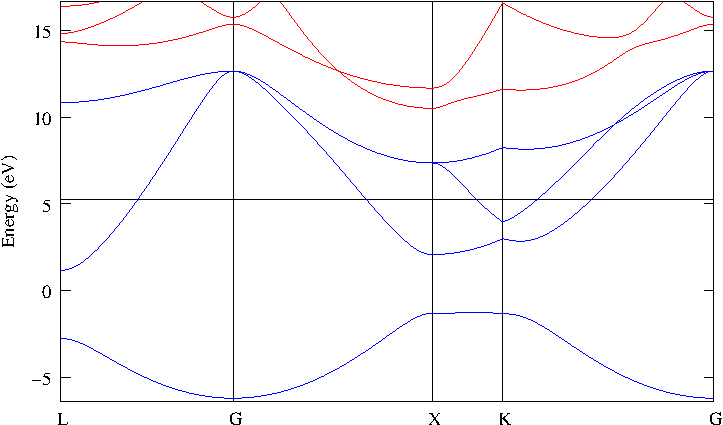
\includegraphics[scale=0.8]{figure/example02/lead.pdf}
\caption{Bandstructure of lead showing the position of the Fermi level. Only the lowest four bands
are included in the calculation.}\label{fig2.1}
\end{figure}

\begin{figure}[h!]
\centering
\subfloat[Energy spectrum of bands]{\raisebox{+2.2in}{\rotatebox[origin=t]{0}{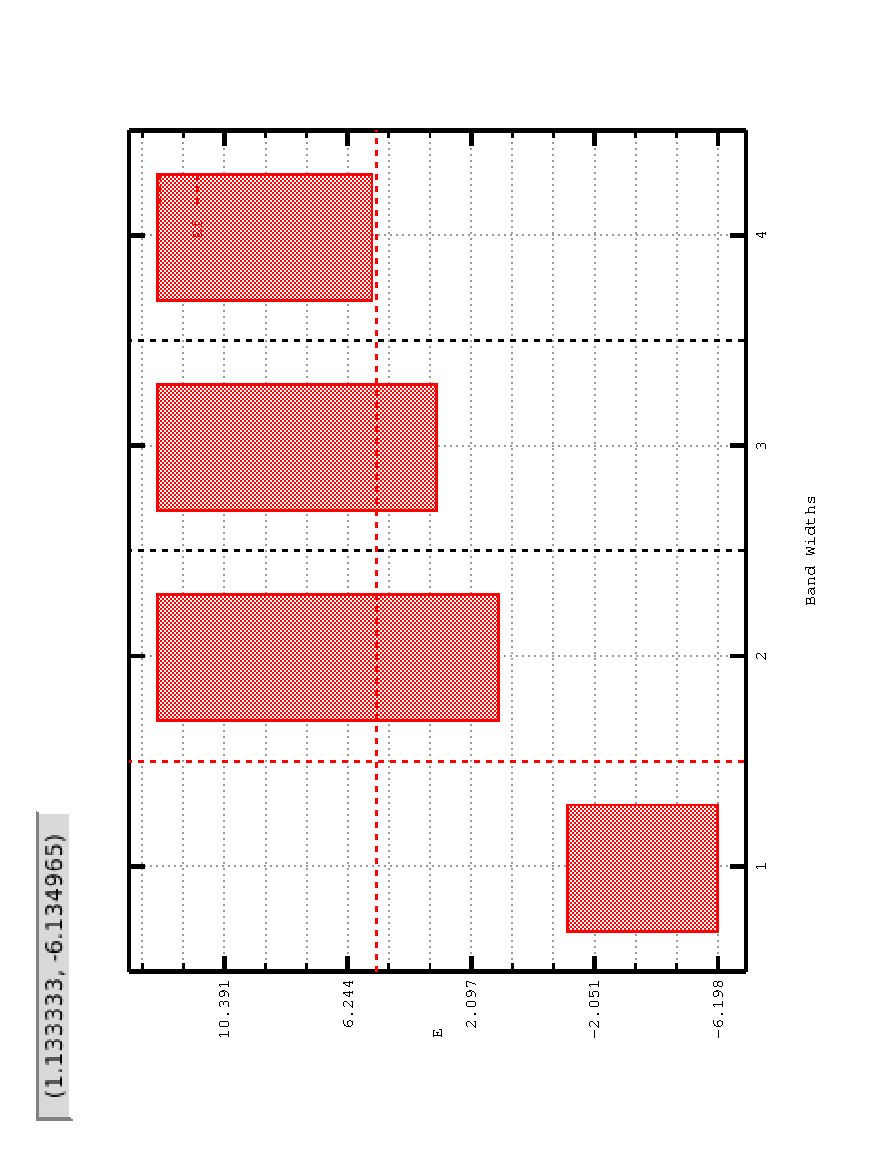
\includegraphics[width=0.33\columnwidth,rotate=270,trim={50pt 0pt 0pt 0pt},clip]{figure/example02/fermi_surface_data_lead.eps}}}}
\centering
\subfloat[band 2]{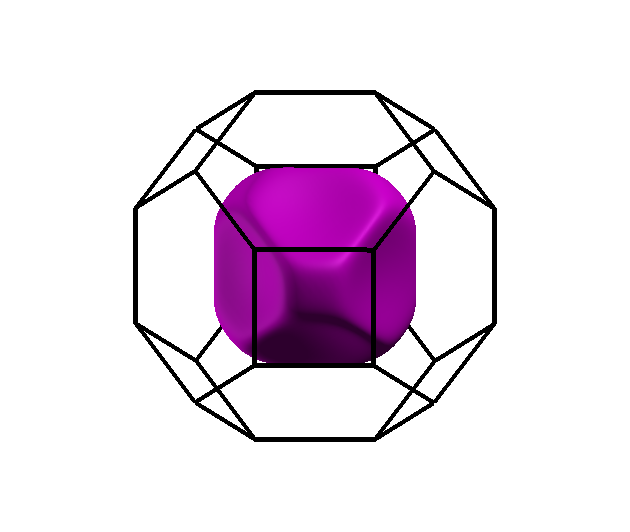
\includegraphics[width=0.25\columnwidth]{figure/example02/lead_band2.png}}
\centering
\subfloat[band 3]{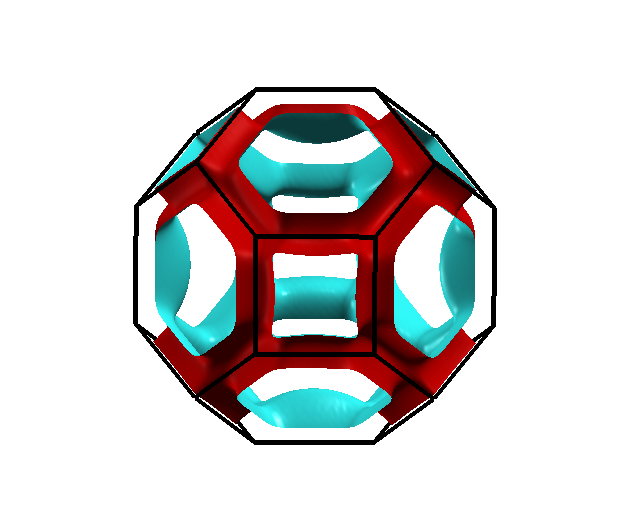
\includegraphics[width=0.25\columnwidth]{figure/example02/lead_band3.png}}
\caption{Fermi surfaces for band 2 and band 3 in lead. The value of the Fermi energy is 5.2676\eV, and it was obtained from the first principle calculation, with a $4\times4\times4$ \bfk-point mesh. To calculate the band energies and to plot Fermi surfaces, Wannier interpolation was employed on a dense mesh in the Brillouin zone consisting of $50^3$ points.}\label{fig2.2}
\end{figure}
\end{enumerate}
